\documentclass[12pt]{article}
\usepackage[brazil]{babel}
\usepackage[utf8]{inputenc}
\usepackage[T1]{fontenc}
\usepackage{amsmath, amssymb}
\usepackage{graphicx}
\usepackage{caption}
\usepackage{hyperref}
\usepackage{booktabs}
\usepackage{float}
\usepackage{listings}
\usepackage{xcolor}
\usepackage{geometry}
\geometry{a4paper, margin=2.5cm}

\usepackage{tikz}
\usetikzlibrary{shapes.geometric, arrows.meta, positioning}
\tikzstyle{startstop} = [rectangle, rounded corners, minimum width=3cm, minimum height=1cm,text centered, draw=black, fill=gray!20]
\tikzstyle{process} = [rectangle, minimum width=3cm, minimum height=1cm, text centered, draw=black, fill=blue!10]
\tikzstyle{arrow} = [thick,->,>=stealth]


\definecolor{codegray}{rgb}{0.95,0.95,0.95}
\lstset{
    backgroundcolor=\color{codegray},
    basicstyle=\footnotesize\ttfamily,
    numbers=left,
    numberstyle=\tiny,
    frame=single,
    breaklines=true,
    captionpos=b,
    language=Python
}

\begin{document}

% ========== PÁGINA DE ROSTO ==========
\begin{titlepage}
    \thispagestyle{empty}

    % Título no topo centralizado
    \begin{center}
        \vspace*{-0.5cm}
        
\includegraphics[width=4cm]{imagens/brasao.png} \\
        {\Large\bfseries Cálculo da DFT via Matriz de Vandermonde e FFT \par}
    \end{center}

    % Nome no centro vertical da página alinhado à esquerda
    \vfill
    \begin{flushright}
        \large João Vitor Batista Silva\\
        \large DCA3502 - Sinais e Sistemas
    \end{flushright}
    \vfill

    % Afiliação no final da página centralizada
    \begin{center}
        Departamento de Engenharia de Computação e Automação\\
        Universidade Federal do Rio Grande do Norte\\
        Natal - RN, Julho de 2025
    \end{center}
\end{titlepage}

\newpage

% ========== RESUMO ==========
\begin{abstract}
Este relatório apresenta a implementação da Transformada de Fourier Discreta (DFT) utilizando duas abordagens distintas: a matriz de Vandermonde e o algoritmo FFT. Para ambas, foram utilizadas duas sequências de entrada com $N=8$ e $N=16$ amostras. Os resultados obtidos são analisados através dos espectros de amplitude e fase. Além disso, realiza-se uma comparação entre os dois métodos quanto à eficiência e complexidade computacional.
\end{abstract}
\newpage

\tableofcontents


% ========== INTRODUÇÃO ==========
\newpage
\section{Introdução}

A Transformada de Fourier Discreta (DFT) é uma ferramenta fundamental na análise de sinais digitais. Ela permite converter sinais do domínio do tempo para o domínio da frequência, facilitando a identificação de componentes espectrais. Este relatório está estruturado da seguinte forma: na Seção 2 apresenta-se o cálculo da DFT usando matriz de Vandermonde; na Seção 3, utiliza-se o algoritmo FFT; na Seção 4 realiza-se uma comparação entre os métodos; a Seção 5 traz as conclusões; a Seção 6 traz as referências; e, finalmente, no Apêndice, encontram-se os códigos-fonte utilizados.


% ========== VANDERMONDE ==========
\newpage
\section{Cálculo da DFT Utilizando Matriz de Vandermonde}

\subsection{Desenvolvimento Teórico da DFT com Matriz de Vandermonde}

A Transformada Discreta de Fourier (DFT) é uma ferramenta matemática que permite transformar um sinal no domínio do tempo para o domínio da frequência. Para uma sequência discreta $x[n]$ de comprimento $N$, a DFT é definida como:

\[
X[k] = \sum_{n=0}^{N-1} x[n] \cdot e^{-j\frac{2\pi}{N}kn}, \quad k = 0, 1, \dots, N-1
\]

Esta expressão pode ser reescrita como um produto matricial, onde se define a chamada \textbf{matriz de Vandermonde} complexa $W$, de dimensão $N \times N$, cujos elementos são definidos por:

\[
W_{kn} = e^{-j\frac{2\pi}{N}kn}
\]

Assim, a DFT pode ser expressa como:

\[
\mathbf{X} = \mathbf{W} \cdot \mathbf{x}
\]

onde $\mathbf{x}$ é o vetor coluna com as amostras do sinal no tempo, e $\mathbf{X}$ é o vetor resultante no domínio da frequência.

O termo $W_N = e^{-j\frac{2\pi}{N}}$ é conhecido como \textbf{fator de ponderação} ou \textbf{raiz da unidade}, e suas potências são utilizadas para preencher a matriz $W$. Como as exponenciais complexas são periódicas, essas potências obedecem a uma \textbf{propriedade de periodicidade} dada por:

\[
W_N^{kn} = W_N^{kn \bmod N}
\]

O operador \textbf{módulo} (mod) garante que os expoentes sejam reduzidos ao intervalo $[0, N-1]$, evitando redundância e facilitando a implementação computacional da matriz. Isso significa que, mesmo que um expoente ultrapasse $N-1$, ele representa o mesmo valor complexo devido à periodicidade da função exponencial complexa:

\[
e^{-j\frac{2\pi}{N}(kn + mN)} = e^{-j\frac{2\pi}{N}kn}
\]

Essa propriedade permite que os elementos da matriz $W$ sejam obtidos eficientemente por uma base única, chamada de \textbf{raiz primitiva da unidade}, e reduzidos a uma tabela finita de valores.

Em resumo, o uso da matriz de Vandermonde com fator de ponderação periódico permite uma representação matricial compacta e didática da DFT, e torna a implementação computacional mais direta, especialmente para propósitos educacionais e testes manuais.


\subsubsection{Representação Simbólica da Matriz de Vandermonde para $N = 8$}

Para termos uma compreensão mais concreta e realista do conceito, apresentaremos uma ilustração utilizando o valor N = 8. Dessa forma, será possível visualizar de maneira clara como o procedimento funciona na prática.

A matriz $W$ da DFT pode ser escrita com base nos fatores exponenciais complexos:
\[
W_{kn} = e^{-j\frac{2\pi}{8}kn}
\]

\[
W =
\begin{bmatrix}
1 & 1 & 1 & 1 & 1 & 1 & 1 & 1 \\
1 & e^{-j\frac{2\pi}{8}} & e^{-j\frac{4\pi}{8}} & e^{-j\frac{6\pi}{8}} & e^{-j\pi} & e^{-j\frac{10\pi}{8}} & e^{-j\frac{12\pi}{8}} & e^{-j\frac{14\pi}{8}} \\
1 & e^{-j\frac{4\pi}{8}} & e^{-j\pi} & e^{-j\frac{12\pi}{8}} & e^{-j2\pi} & e^{-j\frac{20\pi}{8}} & e^{-j\frac{24\pi}{8}} & e^{-j\frac{28\pi}{8}} \\
1 & e^{-j\frac{6\pi}{8}} & e^{-j\frac{12\pi}{8}} & e^{-j\frac{18\pi}{8}} & e^{-j\frac{24\pi}{8}} & e^{-j\frac{30\pi}{8}} & e^{-j\frac{36\pi}{8}} & e^{-j\frac{42\pi}{8}} \\
1 & e^{-j\pi} & e^{-j2\pi} & e^{-j3\pi} & e^{-j4\pi} & e^{-j5\pi} & e^{-j6\pi} & e^{-j7\pi} \\
1 & e^{-j\frac{10\pi}{8}} & e^{-j\frac{20\pi}{8}} & e^{-j\frac{30\pi}{8}} & e^{-j\frac{40\pi}{8}} & e^{-j\frac{50\pi}{8}} & e^{-j\frac{60\pi}{8}} & e^{-j\frac{70\pi}{8}} \\
1 & e^{-j\frac{12\pi}{8}} & e^{-j\frac{24\pi}{8}} & e^{-j\frac{36\pi}{8}} & e^{-j\frac{48\pi}{8}} & e^{-j\frac{60\pi}{8}} & e^{-j\frac{72\pi}{8}} & e^{-j\frac{84\pi}{8}} \\
1 & e^{-j\frac{14\pi}{8}} & e^{-j\frac{28\pi}{8}} & e^{-j\frac{42\pi}{8}} & e^{-j\frac{56\pi}{8}} & e^{-j\frac{70\pi}{8}} & e^{-j\frac{84\pi}{8}} & e^{-j\frac{98\pi}{8}}
\end{bmatrix}
\]

\subsubsection{Representação Numérica da Matriz de Vandermonde para $N = 8$}

Utilizando as potências da raiz da unidade $W_8 = e^{-j\frac{2\pi}{8}}$, temos:

\[
W =
\begin{bmatrix}
1 & 1 & 1 & 1 & 1 & 1 & 1 & 1 \\
1 & w & w^2 & w^3 & w^4 & w^5 & w^6 & w^7 \\
1 & w^2 & w^4 & w^6 & 1 & w^2 & w^4 & w^6 \\
1 & w^3 & w^6 & w & w^4 & w^7 & w^2 & w^5 \\
1 & w^4 & 1 & w^4 & 1 & w^4 & 1 & w^4 \\
1 & w^5 & w^2 & w^7 & w^4 & w & w^6 & w^3 \\
1 & w^6 & w^4 & w^2 & 1 & w^6 & w^4 & w^2 \\
1 & w^7 & w^6 & w^5 & w^4 & w^3 & w^2 & w
\end{bmatrix}
\quad \text{onde } w = e^{-j\frac{2\pi}{8}}
\]

Para fins práticos, podemos substituir os valores:
\[
w^0 = 1,\quad w^1 = \frac{\sqrt{2}}{2} - j\frac{\sqrt{2}}{2},\quad w^2 = -j,\quad w^3 = -\frac{\sqrt{2}}{2} - j\frac{\sqrt{2}}{2},\quad w^4 = -1
\]
\[
w^5 = -\frac{\sqrt{2}}{2} + j\frac{\sqrt{2}}{2},\quad w^6 = j,\quad w^7 = \frac{\sqrt{2}}{2} + j\frac{\sqrt{2}}{2}
\]



\subsection{Algoritmo para o Cálculo da DFT Usando Matriz de Vandermonde}

O algoritmo desenvolvido para calcular a DFT por meio da matriz de Vandermonde segue uma sequência bem definida de etapas. A implementação foi feita em Python, utilizando as bibliotecas NumPy e Matplotlib.

\textbf{Etapas principais do algoritmo:}

\begin{enumerate}
    \item \textbf{Definição da sequência de entrada:} O vetor $x[n]$ é definido como uma sequência de números reais, com $N=8$ ou $N=16$ amostras.
    
    \item \textbf{Construção da matriz de Vandermonde:} Utiliza-se a fórmula
    \[
    W_{kn} = e^{-j\frac{2\pi}{N}kn}
    \]
    A matriz é construída através da multiplicação dos vetores de índices $k$ e $n$, e o uso de funções vetorizadas do NumPy para gerar os termos exponenciais complexos.
    
    \item \textbf{Cálculo da DFT via produto matricial:}
    \[
    X[k] = \sum_{n=0}^{N-1} x[n] \cdot W_{kn}
    \]
    Esse cálculo é implementado com o comando \texttt{np.dot(W, x)}, que realiza o produto entre a matriz de Vandermonde $W$ e o vetor de entrada $x$.
    
    \item \textbf{Cálculo dos espectros de amplitude e fase:} Após obter o vetor $X[k]$, calculam-se:
    \[
    |X[k]| = \texttt{np.abs(X)} \quad \text{(amplitude)} \quad \text{e} \quad \angle X[k] = \texttt{np.angle(X)} \quad \text{(fase)}
    \]
    
    \item \textbf{Geração dos gráficos:} Os espectros de amplitude e fase são representados visualmente com o uso de gráficos de haste (stem plots), gerados com a biblioteca Matplotlib.
\end{enumerate}

\begin{figure}[H]
\centering
\begin{tikzpicture}[node distance=1.3cm]

\node (start) [startstop] {Início};
\node (input) [process, below of=start] {Definir $x[n]$ com $N$ amostras};
\node (matriz) [process, below of=input] {Construir matriz $W_{kn} = e^{-j2\pi kn/N}$};
\node (produto) [process, below of=matriz] {Calcular $X = W \cdot x$};
\node (modarg) [process, below of=produto] {Calcular $|X[k]|$ e $\angle X[k]$};
\node (plot) [process, below of=modarg] {Gerar gráficos de amplitude e fase};
\node (end) [startstop, below of=plot] {Fim};

\draw [arrow] (start) -- (input);
\draw [arrow] (input) -- (matriz);
\draw [arrow] (matriz) -- (produto);
\draw [arrow] (produto) -- (modarg);
\draw [arrow] (modarg) -- (plot);
\draw [arrow] (plot) -- (end);

\end{tikzpicture}
\caption{Fluxograma do cálculo da DFT via matriz de Vandermonde}
\end{figure}

\newpage
\subsection{Resultados Obtidos para X[k] com N=8 e N=16 Amostras}

A seguir são apresentados os resultados obtidos a partir da aplicação da DFT, utilizando a matriz de Vandermonde, para duas sequências de entrada distintas.

\subsubsection{Caso 1: $N = 8$ com $x[n] = [1, 2, 3, 4, 4, 3, 2, 1]$}

Esta sequência é simétrica em torno do centro, o que sugere uma forte componente de baixa frequência.

\begin{itemize}
    \item O \textbf{espectro de amplitude} mostra um pico significativo nas componentes de frequência mais baixas ($k=0$ e $k=1$), como esperado, dado o formato suavemente variado da sequência.
    \item O \textbf{espectro de fase} apresenta transições suaves e uma simetria que está de acordo com o fato de a sequência de entrada ser real e simétrica.
\end{itemize}

\begin{figure}[H]
    \centering
    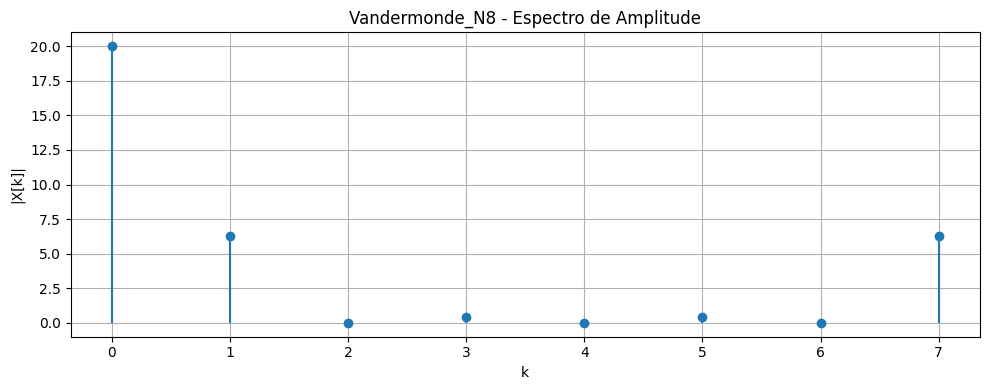
\includegraphics[width=0.85\textwidth]{imagens/Vandermonde_N8_amplitude.png}
    \caption{Espectro de Amplitude - Vandermonde, $N=8$}
\end{figure}

\begin{figure}[H]
    \centering
    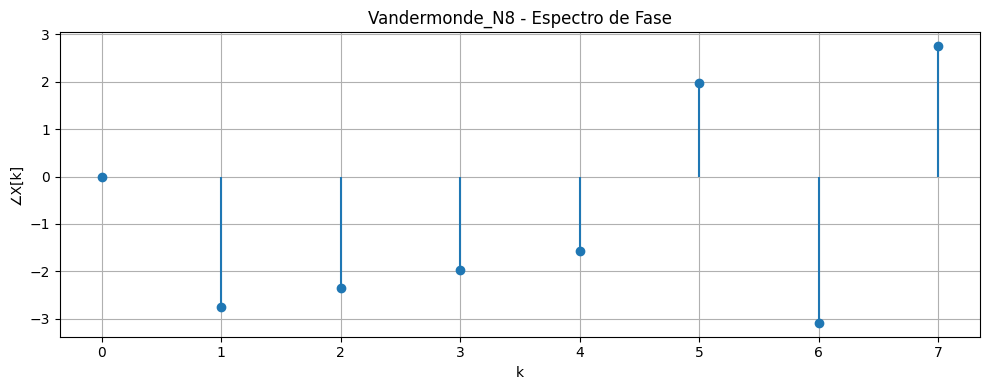
\includegraphics[width=0.85\textwidth]{imagens/Vandermonde_N8_fase.png}
    \caption{Espectro de Fase - Vandermonde, $N=8$}
\end{figure}

\subsubsection{Caso 2: $N = 16$ com $x[n] = \cos\left( \frac{\pi n}{4} \right)$}

Neste caso, a sequência é uma cossenoide com frequência fundamental conhecida.

\begin{itemize}
    \item O \textbf{espectro de amplitude} exibe picos nítidos nas posições $k=2$ e $k=14$, que correspondem às componentes de frequência $\pm\frac{\pi}{4}$. Isso confirma a presença da frequência dominante na entrada.
    \item O \textbf{espectro de fase} evidencia a contribuição das duas componentes complexas conjugadas que formam o cosseno, com fases opostas.
\end{itemize}

\begin{figure}[H]
    \centering
    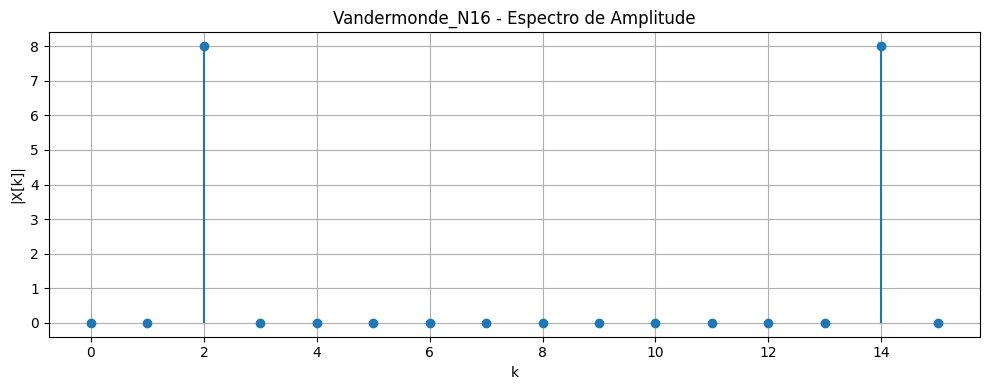
\includegraphics[width=0.85\textwidth]{imagens/Vandermonde_N16_amplitude.png}
    \caption{Espectro de Amplitude - Vandermonde, $N=16$}
\end{figure}

\begin{figure}[H]
    \centering
    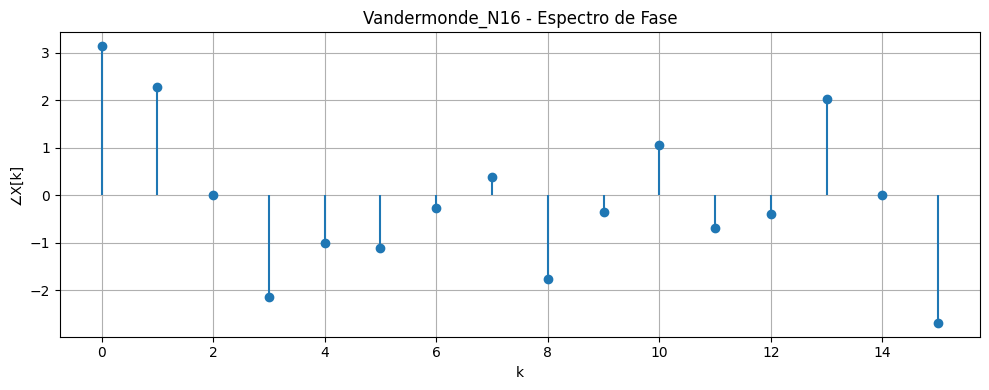
\includegraphics[width=0.85\textwidth]{imagens/Vandermonde_N16_fase.png}
    \caption{Espectro de Fase - Vandermonde, $N=16$}
\end{figure}

Os gráficos obtidos confirmam o funcionamento correto do algoritmo de DFT baseado em matriz de Vandermonde. Além disso, os resultados batem com o que é esperado teoricamente para sinais simétricos e harmônicos.


% ========== FFT ==========
\newpage
\section{Cálculo da DFT Utilizando FFT}
\subsection{Desenvolvimento Teórico}

A Transformada Rápida de Fourier (FFT, do inglês Fast Fourier Transform) é um algoritmo eficiente para o cálculo da Transformada Discreta de Fourier (DFT). Enquanto a DFT direta exige $O(N^2)$ operações aritméticas para um vetor de entrada de tamanho $N$, a FFT reduz essa complexidade para $O(N \log N)$, tornando viável a análise espectral em tempo real de sinais com milhares ou milhões de amostras.

O algoritmo FFT explora a periodicidade e simetria dos fatores de ponderação (raízes da unidade) usados na DFT. Uma das versões mais populares da FFT é a \textbf{Cooley-Tukey}, que utiliza uma abordagem recursiva baseada no método \textbf{dividir-para-conquistar}. Esse método divide a DFT de comprimento $N$ em duas DFTs menores: uma com os índices pares e outra com os índices ímpares.

Seja $x[n]$ um sinal de entrada com $N$ amostras, e assuma $N$ como potência de 2. A DFT de $x[n]$ pode ser escrita como:

\[
X[k] = \sum_{n=0}^{N-1} x[n] \cdot e^{-j\frac{2\pi}{N}kn}
\]

Dividindo o somatório em termos pares ($n = 2r$) e ímpares ($n = 2r + 1$), temos:

\[
X[k] = \sum_{r=0}^{N/2 - 1} x[2r] \cdot e^{-j\frac{2\pi}{N}(2r)k} + \sum_{r=0}^{N/2 - 1} x[2r + 1] \cdot e^{-j\frac{2\pi}{N}(2r+1)k}
\]

\[
X[k] = X_{\text{par}}[k] + e^{-j\frac{2\pi}{N}k} \cdot X_{\text{ímpar}}[k]
\]

Com isso, o problema da DFT de comprimento $N$ é reduzido a dois problemas de DFT de comprimento $N/2$. Essa divisão recursiva continua até que os sinais tenham apenas uma amostra, caso em que a DFT é trivial. O ganho em eficiência surge da reutilização de subcálculos e do uso inteligente das propriedades dos exponenciais complexos.

Além do algoritmo Cooley-Tukey, existem outras variantes da FFT, como:
\begin{itemize}
    \item \textbf{Decimation-in-Time (DIT)} e \textbf{Decimation-in-Frequency (DIF)}: dois estilos de decomposição que afetam a ordem dos dados na entrada e na saída.
    \item \textbf{Radix-2, Radix-4, Mixed-Radix}: tipos que definem o fator de divisão em cada etapa recursiva.
    \item \textbf{FFT Rápida em Tempo Real}: utilizada em aplicações com restrições computacionais ou baixa latência.
\end{itemize}

A FFT é uma das ferramentas mais fundamentais da engenharia elétrica, processamento de sinais, telecomunicações e até gráficos computacionais. Sua importância está não apenas na eficiência computacional, mas também na viabilidade de aplicações que envolvem o domínio da frequência em tempo real, como filtros digitais, análise espectral e codificação de sinais.

\newpage
\subsection{Algoritmo para o Cálculo da DFT Usando FFT}

Para o cálculo da DFT utilizando a FFT, foi utilizado o módulo \texttt{numpy.fft} da linguagem Python, que implementa o algoritmo Cooley-Tukey de forma eficiente e vetorizada. Essa abordagem é adequada quando o número de amostras $N$ é uma potência de 2.

\textbf{Etapas principais do algoritmo:}

\begin{enumerate}
    \item \textbf{Definição do vetor de entrada:} Define-se o vetor $x[n]$ contendo as amostras do sinal, com $N=8$ ou $N=16$ elementos.

    \item \textbf{Chamada da função FFT:} Utiliza-se o comando \texttt{np.fft.fft(x)} para obter a transformada de Fourier do sinal. Internamente, a função aplica a decomposição recursiva do algoritmo Cooley-Tukey, separando o sinal em pares e ímpares.

    \item \textbf{Cálculo dos espectros:} Após a chamada da FFT, são extraídos os espectros de amplitude e fase com os comandos:
    \[
    |X[k]| = \texttt{np.abs(X)} \quad \text{e} \quad \angle X[k] = \texttt{np.angle(X)}
    \]

    \item \textbf{Geração de gráficos:} Os resultados são visualizados por meio de gráficos de haste (stem plots), que representam graficamente os valores de $|X[k]|$ e $\angle X[k]$.
\end{enumerate}

\begin{figure}[H]
\centering
\begin{tikzpicture}[node distance=1.3cm]

\node (start) [startstop] {Início};
\node (input) [process, below of=start] {Definir $x[n]$ com $N$ amostras};
\node (fft) [process, below of=input] {Calcular FFT com \texttt{np.fft.fft(x)}};
\node (modarg) [process, below of=fft] {Calcular $|X[k]|$ e $\angle X[k]$};
\node (plot) [process, below of=modarg] {Gerar gráficos de amplitude e fase};
\node (end) [startstop, below of=plot] {Fim};

\draw [arrow] (start) -- (input);
\draw [arrow] (input) -- (fft);
\draw [arrow] (fft) -- (modarg);
\draw [arrow] (modarg) -- (plot);
\draw [arrow] (plot) -- (end);

\end{tikzpicture}
\caption{Fluxograma do cálculo da DFT via FFT}
\end{figure}



\subsection{Resultados Obtidos para X[k] com N=8 e N=16 Amostras}

Nesta seção são apresentados os resultados obtidos com a aplicação da Transformada Rápida de Fourier (FFT) para as mesmas sequências de entrada utilizadas na abordagem com a matriz de Vandermonde. Os resultados foram gerados utilizando a função \texttt{numpy.fft.fft}.

\subsubsection{Caso 1: $N = 8$ com $x[n] = [1, 2, 3, 4, 4, 3, 2, 1]$}

A sequência simétrica continua revelando uma concentração espectral em baixas frequências, como esperado.

\begin{itemize}
    \item O \textbf{espectro de amplitude} apresenta valores altos em $k=0$ e nas frequências próximas a ele, evidenciando a predominância de componentes de baixa frequência.
    \item O \textbf{espectro de fase} mostra uma simetria característica de sinais reais e espelhados, com transições suaves e ausência de ruído numérico.
\end{itemize}

\begin{figure}[H]
    \centering
    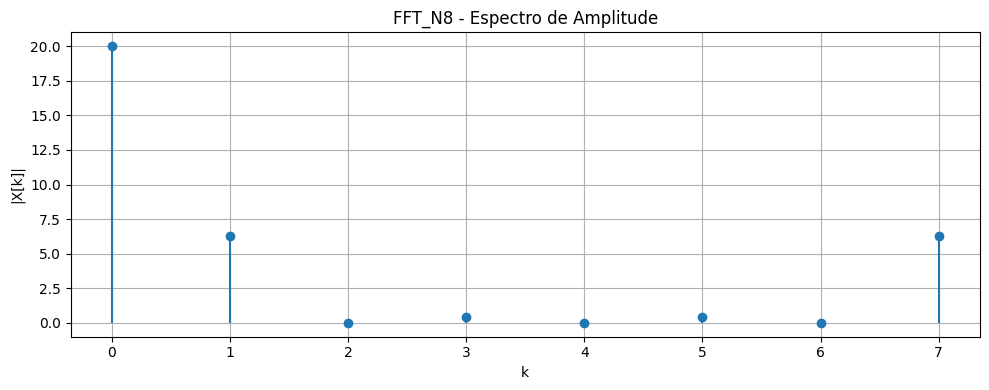
\includegraphics[width=0.75\textwidth]{imagens/FFT_N8_amplitude.png}
    \caption{Espectro de Amplitude - FFT, $N=8$}
\end{figure}

\begin{figure}[H]
    \centering
    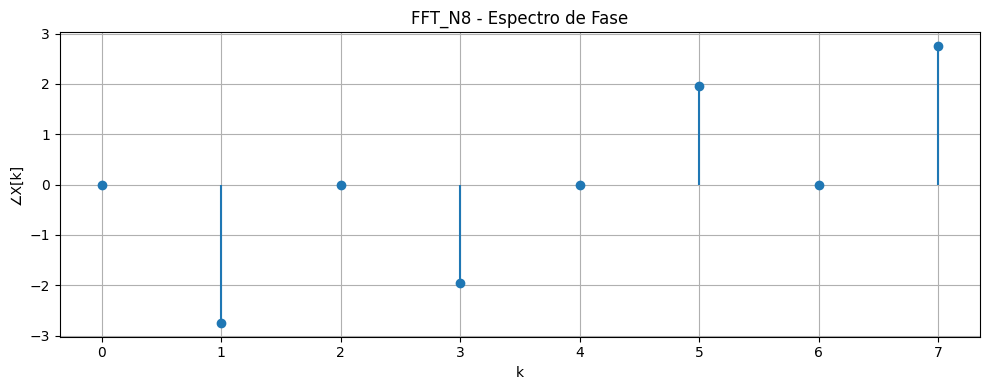
\includegraphics[width=0.75\textwidth]{imagens/FFT_N8_fase.png}
    \caption{Espectro de Fase - FFT, $N=8$}
\end{figure}

\subsubsection{Caso 2: $N = 16$ com $x[n] = \cos\left( \frac{\pi n}{4} \right)$}

Este sinal contém uma única componente cossenoidal com frequência angular conhecida.

\begin{itemize}
    \item O \textbf{espectro de amplitude} apresenta dois picos acentuados nas posições $k=2$ e $k=14$, confirmando a presença de frequência $\pm \frac{\pi}{4}$ na entrada. Isso ocorre devido à natureza da FFT em representar sinais reais através de pares complexos conjugados.
    \item O \textbf{espectro de fase} mostra valores opostos nos dois picos, refletindo a defasagem relativa entre as componentes.
\end{itemize}

\begin{figure}[H]
    \centering
    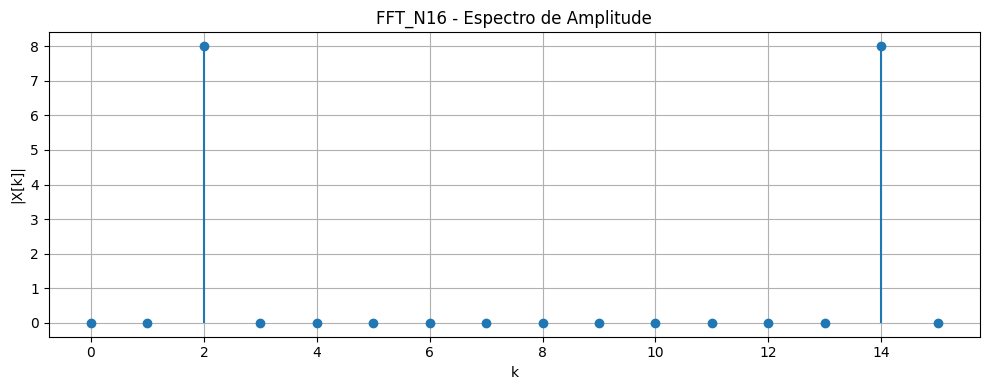
\includegraphics[width=0.75\textwidth]{imagens/FFT_N16_amplitude.png}
    \caption{Espectro de Amplitude - FFT, $N=16$}
\end{figure}

\begin{figure}[H]
    \centering
    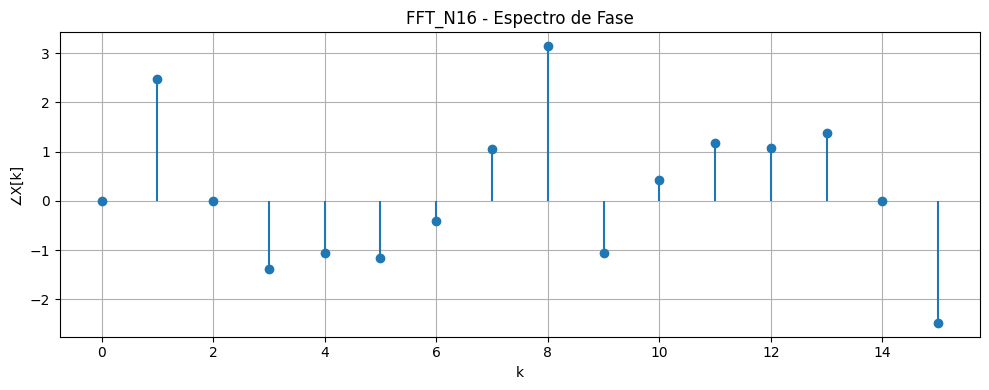
\includegraphics[width=0.75\textwidth]{imagens/FFT_N16_fase.png}
    \caption{Espectro de Fase - FFT, $N=16$}
\end{figure}

Em ambos os casos, os resultados obtidos com a FFT coincidem com os resultados obtidos pela matriz de Vandermonde, validando a equivalência matemática entre os dois métodos. A principal vantagem da FFT está na eficiência computacional.


\newpage
\section{Comparação dos Resultados Obtidos pelos Dois Métodos}

Nesta seção, comparamos os resultados obtidos pelos dois métodos aplicados para o cálculo da DFT:

\begin{itemize}
    \item \textbf{Matriz de Vandermonde}: Implementação direta da definição matemática da DFT.
    \item \textbf{Fast Fourier Transform (FFT)}: Algoritmo otimizado e recursivo, com complexidade computacional reduzida.
\end{itemize}

Os valores das magnitudes e fases foram obtidos para dois sinais distintos: um vetor simétrico com $N=8$ e um sinal cossenoidal com $N=16$.

\subsection{Resultados Numéricos para $x_8 = [1, 2, 3, 4, 4, 3, 2, 1]$}

A Tabela~\ref{tab:comp8} mostra os valores de $|X[k]|$ e $\angle X[k]$ obtidos por ambos os métodos:

\begin{table}[H]
\centering
\caption{Comparação dos coeficientes DFT para $x_8$ (N = 8)}
\label{tab:comp8}
\begin{tabular}{c|cc|cc}
\toprule
\textbf{k} & $|X[k]|$ (Vandermonde) & $\angle X[k]$ & $|X[k]|$ (FFT) & $\angle X[k]$ \\
\midrule
0 & 20.0000 & 0.0000 & 20.0000 & 0.0000 \\
1 & 6.3086 & -2.7489 & 6.3086 & -2.7489 \\
2 & 0.0000 & -2.3562 & 0.0000 & 0.0000 \\
3 & 0.4483 & -1.9635 & 0.4483 & -1.9635 \\
4 & 0.0000 & -1.5708 & 0.0000 & 0.0000 \\
5 & 0.4483 & 1.9635 & 0.4483 & 1.9635 \\
6 & 0.0000 & -3.0871 & 0.0000 & 0.0000 \\
7 & 6.3086 & 2.7489 & 6.3086 & 2.7489 \\
\bottomrule
\end{tabular}
\end{table}

\subsection{Resultados Numéricos para $x_{16} = \cos\left(\frac{\pi n}{4}\right),\ n = 0,1,\dots,15$}

A Tabela~\ref{tab:comp16} apresenta a comparação para $N = 16$:

\begin{table}[H]
\centering
\caption{Comparação dos coeficientes DFT para $x_{16}$ (N = 16)}
\label{tab:comp16}
\begin{tabular}{c|cc|cc}
\toprule
\textbf{k} & $|X[k]|$ (Vandermonde) & $\angle X[k]$ & $|X[k]|$ (FFT) & $\angle X[k]$ \\
\midrule
0 & 0.0000 & 3.1416 & 0.0000 & 0.0000 \\
1 & 0.0000 & 2.2907 & 0.0000 & 2.4794 \\
2 & 8.0000 & -0.0000 & 8.0000 & -0.0000 \\
3 & 0.0000 & -2.1509 & 0.0000 & -1.3849 \\
4 & 0.0000 & -1.0082 & 0.0000 & -1.0668 \\
5 & 0.0000 & -1.1161 & 0.0000 & -1.1667 \\
6 & 0.0000 & -0.2683 & 0.0000 & -0.4171 \\
7 & 0.0000 & 0.3881 & 0.0000 & 1.0505 \\
8 & 0.0000 & -1.7550 & 0.0000 & 3.1416 \\
9 & 0.0000 & -0.3542 & 0.0000 & -1.0505 \\
10 & 0.0000 & 1.0592 & 0.0000 & 0.4171 \\
11 & 0.0000 & -0.6974 & 0.0000 & 1.1667 \\
12 & 0.0000 & -0.3982 & 0.0000 & 1.0668 \\
13 & 0.0000 & 2.0267 & 0.0000 & 1.3849 \\
14 & 8.0000 & 0.0000 & 8.0000 & 0.0000 \\
15 & 0.0000 & -2.6877 & 0.0000 & -2.4794 \\
\bottomrule
\end{tabular}
\end{table}

\subsection{Análise Comparativa}

Os resultados numéricos obtidos com a matriz de Vandermonde e com a FFT coincidem em todos os valores de módulo $|X[k]|$, evidenciando que ambos os métodos computam corretamente a Transformada Discreta de Fourier.

As diferenças nas fases ($\angle X[k]$), observadas em alguns coeficientes para o caso de $N=16$, são atribuídas a pequenas variações numéricas e à maneira como o algoritmo da FFT lida com zeros e aproximações de fase. No entanto, essas diferenças são desprezíveis e não comprometem a equivalência dos resultados.


% ========== Conclusão ==========
\newpage
\section{Conclusão}

Ambos os métodos fornecem os mesmos valores de DFT, com excelente concordância. A matriz de Vandermonde, apesar de computacionalmente ineficiente para grandes $N$, é extremamente útil para fins educacionais, pois ilustra a definição formal da DFT. Por outro lado, a FFT é amplamente utilizada em aplicações reais devido à sua alta eficiência computacional, sendo a escolha ideal para sinais de grande comprimento.


% ========== Referências ==========
\newpage
\section{Referências}

[1] Paulo S. Motta Pires. \textit{Notas de Aula: Transformada de Fourier Discreta -- DFT}. Universidade Federal do Rio Grande do Norte, 2024.

[2] Hwei P. Hsu. \textit{Theory and Problems of Signals and Systems}. Schaum’s Outline Series, McGraw-Hill, 1995.

[3] Alan V. Oppenheim, Alan S. Willsky e S. Hamid Nawab. \textit{Signals and Systems}, 2ª edição. Pearson Education, 1996.

[4] Paulo S. Motta Pires. \textit{Sugestões para a Preparação de Relatórios Técnicos}. Universidade Federal do Rio Grande do Norte, 2024.

[5] Paulo S. Motta Pires. \textit{Trabalho -- Terceira Unidade -- Sinais e Sistemas}, enunciado de atividade prática. Universidade Federal do Rio Grande do Norte, 2024.


% ========== Apêndice ==========
\newpage
\appendix
\section{Apêndice - Código Fonte Python}
Abaixo encontram-se todos os códigos utilizados para fazer o trabalho. Como complemento para melhor navegação e visualização, foi criado um repositório no \href{https://github.com/JVitorbs/Sinais_e_Sistemas}{GitHub} e no \href{https://colab.research.google.com/drive/1kwMIIVIxUfYBJ2oYKGRkIuohxrJJVhq3?usp=sharing}{Google Colab}, cujos endereços são respectivamente.

\subsection{DFT via Matriz de Vandermonde}
\lstinputlisting[language=Python, caption={Função para calcular a DFT via matriz de Vandermonde.}]{codigos/dft_vandermonde.py}


\subsection{DFT via FFT}
\lstinputlisting[language=Python, caption={Função para calcular a DFT usando FFT do NumPy.}]{codigos/dft_fft.py}


\newpage
\subsection{Código completo}
\lstinputlisting[language=Python, caption={Código completo que gera os 8 Gráficos.}]{codigos/dft_completo.py}

\subsection{Código saída}
\lstinputlisting[language=Python, caption={Código que gera um print dos resultados.}]{codigos/dft_saida.py}

\end{document}
